\documentclass[./00PhotoBox.tex]{subfiles}
\graphicspath{{\subfix{./img/}}}
\begin{document}

\chapter{Untersuchungen zur Genauigkeit und Systemaufbau}
\label{c:versuche}
Nach Abschluss der Konstruktion und des Aufbaus des Prototyps, wurden verschiedene Untersuchungen durchgeführt, um die Genauigkeit des Systems zu überprüfen und die Anzahl der Kameras zu evaluieren. Hierzu wurden unter anderem Vergleichsmessungen mit verschiedenen Systemen durchgeführt.

\section{Referenzdaten}
\label{s:referenzdaten}
Zum Vergleich standen verschiedene Testobjekte zur Verfügung. Hauptsächlich wurde ein etwa \SI{14}{\centi\metre} hohes Modell einer Moai-Statue der Osterinsel verwendet, da dieses Objekt eine gute Textur und viele Details aufweist (siehe \autoref{img:bild_moai}). Neben einem texturierten Spielzeugdino standen noch zwei weiße Gipsmodelle zur Verfügung: Ein Abdruck einer Büste Einsteins  (siehe \autoref{img:bild_einstein}) und ein kerzenartiges Testobjekt, im folgenden Testy genannt (siehe \autoref{img:bild_testy}). Alle Objekte wurden bereits in anderen Projekten an der HafenCity Universität verwendet \citep[z.\,B.][]{kersten_scanner} und sind mit mehreren verschiedenen Systemen vermessen worden.

\begin{figure}
    \centering
    \begin{subfigure}{0.32\textwidth}
        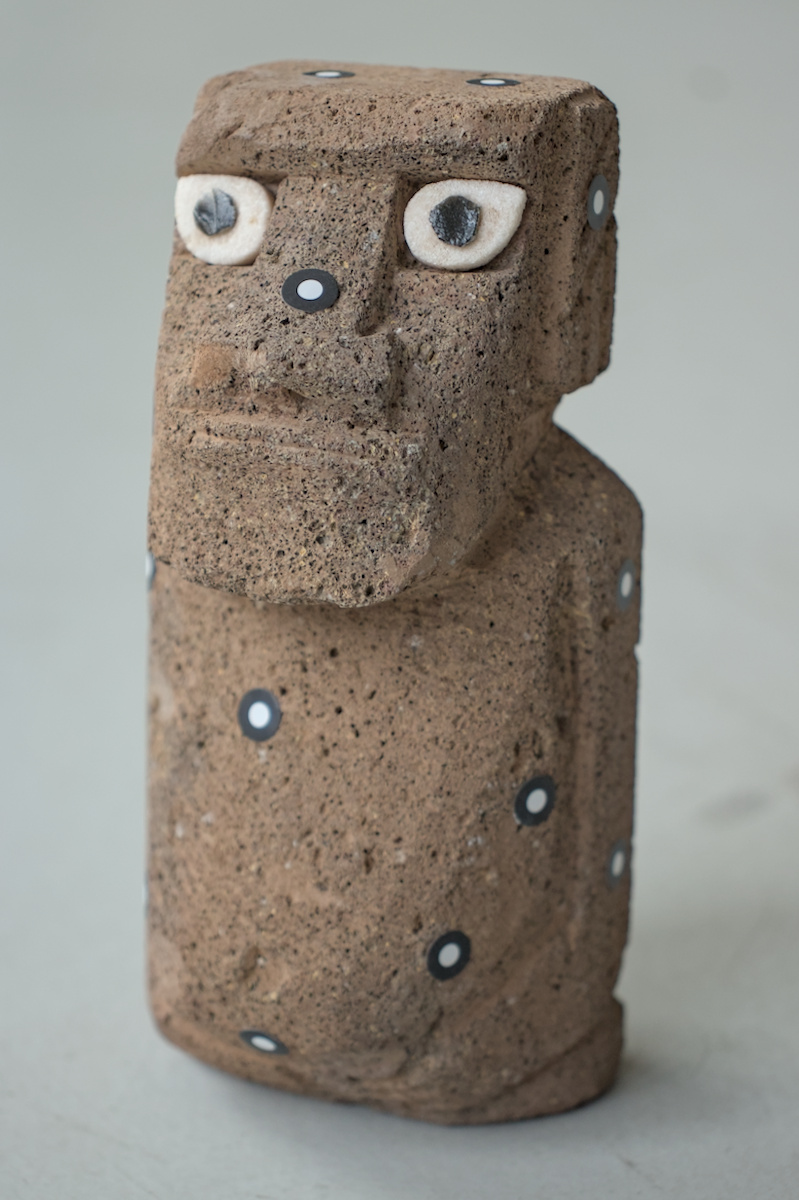
\includegraphics[width=1\textwidth]{img/7_versuche/bild_moai.jpg}
        \caption{Moai}
        \label{img:bild_moai}
    \end{subfigure}
    \begin{subfigure}{0.32\textwidth}
        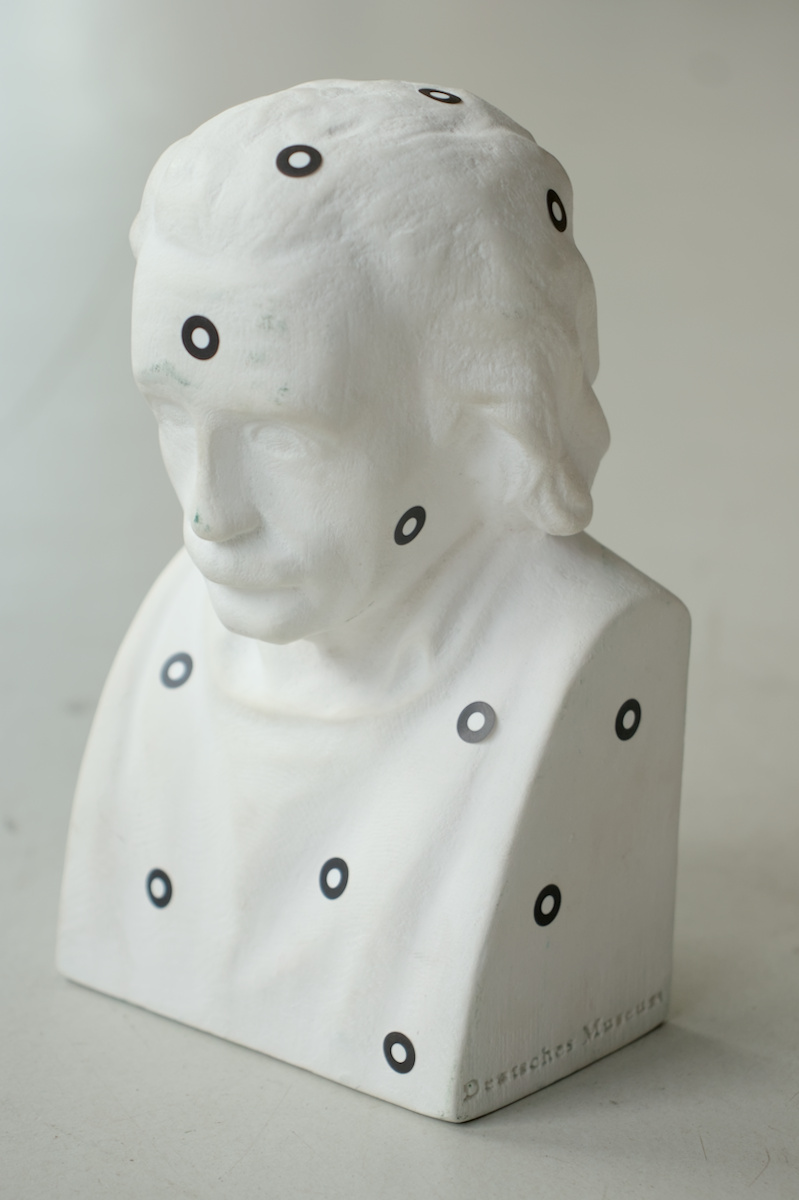
\includegraphics[width=1\textwidth]{img/7_versuche/bild_einstein.jpg}
        \caption{Einstein}
        \label{img:bild_einstein}
    \end{subfigure}
    \begin{subfigure}{0.32\textwidth}
        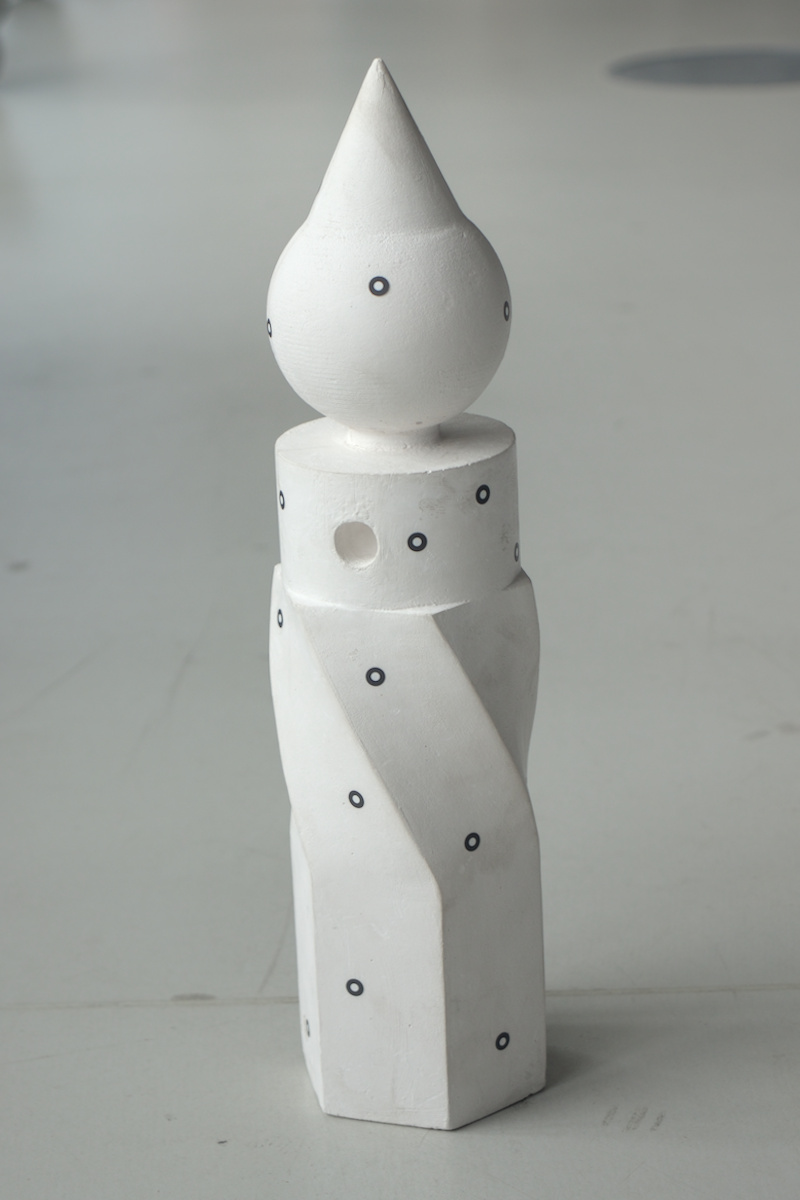
\includegraphics[width=1\textwidth]{img/7_versuche/bild_testy.jpg}
        \caption{Testy}
        \label{img:bild_testy}
    \end{subfigure}
    \caption{Verschiedene Testobjekte}
    \label{img:bilder_testobjekte}
\end{figure}

Als Referenzwerte wurden in dieser Arbeit die Messungen mit einem Zeiss GOM ATOS 5 genutzt. Hierbei handelt es sich um ein Streifenprojektionssystem, welches hauptsächlich in der Industrie zur Vermessung von Bauteilen eingesetzt wird. Streifenprojektionssysteme arbeiten auch photogrammetrisch, haben aber den Vorteil, das sie durch das Projektionssystem auch texturarme Objekte erfassen können. Wie der Name bereits andeutet, wird ein Streifenmuster auf das Objekt projiziert, welches dann von mindestens einer Kamera aufgenommen wird. Projektor und Kamera sind auf einer festen Basis montiert. \citep[S. 581f]{luhmann}

Bei dem verwendeten System werden zwei Kameras eingesetzt, die sich ein massives Gehäuse mit dem mittig angeordneten Projektor teilen. Je nach verwendeten Messvolumen und Objektentfernung beträgt die Genauigkeit etwa \SI{0,01}{} - \SI{0,03}{\milli\metre} \citep{atos}. Aufgrund der deutlich höheren erwarteten Genauigkeit des Streifenprojektionssystems, kann davon ausgegangen werden, dass die Messungen deutlich genauer sind als die des Prototyps und als quasi-wahre Werte angenommen werden können.

Ausnahmen hiervon stellen die Positionen der Verknüpfungspunkte durch kreisförmige Marker dar. Diese wurden zur Messung mit dem ATOS 5 angebracht, um die verschiedenen Aufnahmen zu verknüpfen. Sie werden vom Streifenprojektionssystem automatisch erkannt, für die Verknüpfung genutzt und die Bereiche im erzeugten 3D-Modell interpoliert. Dadurch können hier größere Abweichungen entstehen, sofern die Oberfläche nicht eben ist oder die Dicke der Passpunktmarken nicht korrekt in der Software des Streifenprojektionssystems angegeben ist.

Die Moai-Figur wurde auch bereits mit einer Spiegelreflexkamera Nikon D90 vermessen. Hierbei wurden manuell Bilder aufgenommen und diese mit Agisoft Metashape ausgewertet. Hiermit steht damit auch ein klassisches photogrammetrisches Modell zur Verfügung.


\section{Vorgehen zur Genauigkeitsüberprüfung}

Das Vorgehen zur Bewertung der erzeugten Daten unterscheidet sich zwischen den verschiedenen Untersuchungen kaum. Dieser Abschnitt beschreibt daher allgemein das Vorgehen und die verwendeten Parameter zur Bewertung der Punktwolken. Außerdem wird eine Abschätzung der erwarteten Genauigkeit des Systems vorgenommen.


\subsection{Erwartete Genauigkeit}
\label{ss:erwartete_genauigkeit}
Die erwartete Genauigkeit kann auf verschiedenen Wegen berechnet werden. Grundlage ist meistens der Bildmaßstab. Dieser unterscheidet sich je nach Entfernung. Die Entfernung zum Objekt beträgt im Normalfall zwischen $10$ und \SI{50}{\centi\metre}. Der Bildmaßstab $m$ berechnet sich nach \cite[S. 171]{luhmann} wie folgt:

\begin{align*}
    \nlabel{eq:bildmassstab}
    m       & = \frac{h}{c}                                                    \\
    m_{min} & = \frac{\SI{100}{\milli\metre}}{\SI{4,7}{\milli\metre}} = 21,28  \\
    m_{max} & = \frac{\SI{500}{\milli\metre}}{\SI{4,7}{\milli\metre}} = 106,38
\end{align*}
\begin{conditions}
    m & Bildmaßstab \\
    h & Abstand zur Kamera \\
    c & \Gls{Kamerakonstante} (\SI{4,7}{\milli\metre})
\end{conditions}

Für die Bildmessgenauigkeit werden verschiedene Werte in der Literatur erwähnt, sie liegen je nach Messmethode zwischen \SI{0,05}{} und $3$\,\gls{px}. Für Messung von \acrshort{CCCT}s wird zum Beispiel von \cite{soot2015} eine Genauigkeit von $0,1$\,\gls{px} angegeben.
Eigene, manuelle Messungen ergaben eine Genauigkeit von etwa $1,5$\,\gls{px}. Vereinfacht wurde mit $1$\,\gls{px} Genauigkeit gerechnet.

Die Bildmessgenauigkeit $dx'$  wird dann mit dem Bildmaßstab multipliziert und ergibt die vorläufige Lagegenauigkeit $dX$ (\autoref{eq:bildmessgenauigkeit}):

\begin{align*}
    dx'      & = \SI{1}{\gls{px}} \cdot \SI{0,0014}{\milli\metre\per px} = \SI{0,0014}{\milli\metre} \\
    \nlabel{eq:bildmessgenauigkeit}
    dX       & = m \cdot dx'                                                                         \\
    dX_{min} & = 21,28 \cdot \SI{0,0014}{\milli\metre} = \SI{0,03}{\milli\metre}                     \\
    dX_{max} & = 106,38 \cdot \SI{0,0014}{\milli\metre} = \SI{0,15}{\milli\metre}
\end{align*}
\begin{conditions}
    dx' & Bildmessgenauigkeit \\
    dX  & Lage-Genauigkeit (Objektraum)
\end{conditions}

An diesem Wert muss dann noch der sogenannte Design-Faktor $q$ angebracht werden. \citet[S. 174]{luhmann} beschreibt diesen als Parameter der Aufnahmegeometrie und den auftretenden Schnitten. Dieser liege bei Rundumverbänden zwischen $0,4$ und $0,8$ und bei Stereoaufnahmen bei $1,5 - 3,0$. Vereinfacht für eine grobe Abschätzung wird hier daher der Faktor weggelassen. Die erwartete Genauigkeit liegt damit deutlich unter einem Millimeter in der Lage.

\begin{align*}
    \nlabel{eq:genauigkeit_lage}
    s_{px; min}' & = dX_{min} \\
    s_{px; max}' & = dX_{max}
\end{align*}

Die Genauigkeit der Tiefeninformationen ist von dem Verhältnis des Abstandes der Kameras zur Entfernung abhängig. Zwischen zwei Kamerareihen sind etwa \SI{25}{\centi\metre} Abstand. Die Genauigkeit der Tiefeninformationen kann daher wie folgt berechnet werden \citep[S. 174]{luhmann}:

\begin{align*}
    \nlabel{eq:genauigkeit_tiefe}
    s_Z       & = m \, \frac{h}{b} \, s_{\gls{px}}'                                                                                        \\
    s_{Z;min} & = 21,28 \cdot \frac{\SI{10}{\centi\metre}}{\SI{30}{\centi\metre}}\cdot \SI{0,03}{\milli\metre}  = \SI{0,02}{\milli\metre}  \\
    s_{Z;max} & = 106,38 \cdot \frac{\SI{50}{\centi\metre}}{\SI{30}{\centi\metre}} \cdot \SI{0,15}{\milli\metre} = \SI{0,25}{\milli\metre}
\end{align*}
\begin{conditions}
    s_Z & Genauigkeit der Tiefeninformationen \\
    b   & Basislinie (hier \SI{30}{\centi\metre})
\end{conditions}

Die erwartete Genauigkeit und auch die Auflösung der Kameras liegt demnach im Bereich eines Fünftel Millimeters.


\subsection{Verwendete Parameter}
\label{ss:verwendete_parameter}
Zum Vergleich der Ergebnisse wurden verschiedene Parameter in den Auswertungen betrachtet. Diese sind im Folgenden kurz erläutert.

\subsubsection{Quasi-wahrer Wert/Fehler}
Die Messung mit dem Streifenprojektionssystem ist nach der Genauigkeitsabschätzung des Prototyps etwa zehnmal genauer. Daher kann das Ergebnis des Streifenprojektionssystems hier als quasi-wahrer Wert angenommen werden \cite[S. 43]{hoepcke}. Der quasi-wahre Fehler ist nach \citet[S. 44, Formel 2-2, siehe \autoref{eq:quasi_wahrer_wert}]{hoepcke} die Differenz zwischen quasi-wahren Wert und der Beobachtung. Im Fall dieser dreidimensionalen Messung wurde der Abstand zwischen einem Punkt der Punktwolken des Prototyps und der Oberfläche aus der Messung des Streifenprojektionssystems als quasi-wahrer Fehler angenommen. Punkte innerhalb des Objektes wurden mit einem negativen Vorzeichen versehen.

\begin{align*}
    \nlabel{eq:quasi_wahrer_wert}
    l + \varepsilon' & = \lambda'
\end{align*}
\begin{conditions}
    l & Beobachtung\\
    \varepsilon' & quasi-wahrer Fehler\\
    \lambda' &  quasi-wahrer Wert
\end{conditions}

\subsubsection{Durchschnittlicher Fehler / Mittelwert des quasi-wahren Fehlers}

Der durchschnittliche Fehler ist der Mittelwert des Betrages des quasi-wahren Fehlers \citep[S.44, Gleichung 2-4, siehe \autoref{eq:durchschnittlicher_fehler}]{hoepcke}. Er gibt an, wie stark die Punktwolke von der Referenz abweicht. Der Mittelwert des quasi-wahren Fehlers (\autoref{eq:mittelwert_quasi_wahrer_fehler}) ist eher unüblich, da sich hier positive und negative Abweichungen aufheben. Da das Vorzeichen mitberücksichtigt wird, zeigt dieser, ob die Punktwolke systematisch zu groß oder zu klein ist, also ob die Realisierung des Maßstabes ungenau war.

\begin{align*}
    \nlabel{eq:durchschnittlicher_fehler}
    t                       & = \frac{1}{n} \sum_{i=1}^{n} \left| \varepsilon'_i \right| \\
    \nlabel{eq:mittelwert_quasi_wahrer_fehler}
    \overline{\varepsilon'} & = \frac{1}{n} \sum_{i=1}^{n}  \varepsilon'_i
\end{align*}


\subsubsection{Mittlerer Fehler}

Der mittlere Fehler ergibt sich aus der Quadratsumme des quasi-wahren Fehlers, geteilt durch die Anzahl der Messungen.  Er ist das wichtigste Maß für die Genauigkeit der Punktwolke \citep[S. 45, Gleichung 2-5b, siehe \autoref{eq:mittlerer_fehler}]{hoepcke}.

\begin{align*}
    \nlabel{eq:mittlerer_fehler}
    m = \sqrt{\frac{1}{n} \sum_{i=1}^{n} \varepsilon_i^2}
\end{align*}


\subsubsection{Maximaler Fehler}

Der maximale Fehler gibt den größten Fehler an, der in der Punktwolke auftritt. Er zeigt, wie stark die Punktwolke von der Referenz abweicht und ob es Ausreißer gibt.



\subsubsection{Punktanzahl}
Die Anzahl der Punkte einer Punktwolke alleine ist kein Maß für die Qualität der Punktwolke. Sie kann zwar als Indikator für die Abdeckung der Oberfläche genutzt werden, jedoch nicht für die Genauigkeit. Die Anzahl der Punkte wurde daher nur als zusätzlicher Parameter betrachtet bzw. aufgrund der Einfachheit der Bestimmung als Hilfsparameter genutzt, welcher durch die beiden folgenden Parameter ergänzt wird.

\subsubsection{Abdeckung}
Als weiterer Kriterium wurde die Abdeckung der Objektoberfläche mit Punkten bewertet. Dazu wurden die Punktwolken auf diejenigen gefiltert, die weniger als einen Millimeter vom Modell des Streifenprojektionssystems entfernt waren. Diese wurden dann auf eine Punktdichte von \SI{1}{\milli\metre} Punktabstand reduziert und die Anzahl der Punkte gezählt. Die Anzahl dieser Punkte wurde mit der genauso bestimmten Anzahl des Referenzdatensatzes in Beziehung gesetzt. Dadurch konnte die Abdeckung der Oberfläche bewertet werden. Eine Abdeckung von \SI{100}{\percent} bedeutet, dass die Punktwolke die Oberfläche des Referenzdatensatzes vollständig abdeckt. Kleinere Werte zeigen an, dass die Oberfläche nicht vollständig erfasst wurde.

\subsubsection{Richtigkeit}
Darüber hinaus wurde die Anzahl der Punkte nach der Ausdünnung bestimmt ohne Nutzung des zuvor beschriebenen Abstandsfilter. Dieser wurde dann mit der Anzahl der Punkte unter Nutzung des Abstandsfilters in Beziehung gesetzt. Dadurch konnte der Anteil der richtig liegenden Punkte unabhängig von der Anzahl der Punkte bewertet werden. Auch hier bedeutet ein Wert von \SI{100}{\percent}, dass alle Punkte richtig bzw. maximal \SI{1}{\milli\metre} von der Oberfläche der Referenzdaten entfernt liegen. Kleinere Werte zeigen an, dass die Punktwolke Ausreißer enthält.




\section{Genauigkeitsüberprüfung des 3D-Modelles}
\label{s:genauigkeitsueberpruefung}
Um die Genauigkeit der 3D-Modell-Erzeugung zu überprüfen, wurden mehrere Prüf\-körper mit dem Prototyp vermessen. Die Ergebnisse wurden anschließend im Vergleich zu dem Streifenprojektionssystem und der Aufnahme des Moais mit einer Spiegelreflexkamera betrachtet.

\subsection{Durchführung}
Alle drei Testobjekte wurden mit dem Prototyp aufgenommen und die Daten in Agisoft Metashape verarbeitet. Die modellierte Oberfläche aus dem Streifenprojektionssystem und die Punktwolke aus dem Prototyp wurden in CloudCompare aufeinandergelegt. Hieraus wurde anschließend die Differenz und die Genauigkeit anhand dieser berechnet.

\subsection{Ergebnisse}
Die Visualisierung der Differenzen ist in \autoref{img:differenz} dargestellt. Es ist zu erkennen, dass je nach Modell einige Bereiche gar nicht erfasst bzw. deren Genauigkeit deutlich von der erwarteten abweichen.

\paragraph{Moai}
Beim Moai (siehe \autoref{img:differenz_moai_einzel}) sind die größten Fehlstellen im Bereich des Kinnes und unterhalb des Bauches zu erkennen. Abweichungen im Bereich des restlichen Körpers sind deutlich geringer und liegen im Bereich von \SI{0,21}{\milli\metre}. Sie sind auf die schlechtere Erfassung der nach unten gerichteten Flächen zurückzuführen. Diese Bildbereiche sind nur in wenigen Bildern sichtbar und können daher nicht so gut rekonstruiert werden. Weitere Abweichungen sind im Bereich der Passpunktmarken zu erkennen, hier ist unklar, welche Daten korrekt sind (vgl. \autoref{s:referenzdaten}).


\paragraph{Einstein}
Das Modell von Einstein (siehe \autoref{img:differenz_einstein}) zeigt ebenfalls größere Abweichungen im Bereich des Kinnes und des Halses. Die Passpunktmarken sind zwar auch in der Differenzdarstellung erkennbar, jedoch nicht mit so großen Abweichungen wie beim Moai. Im Gegensatz zum Moai sind die Abweichungen im Bereich des Kopfes und der Schultern deutlich großflächiger. Gerade die großen weißen, texturarmen Flächen führen jedoch zu schlechteren Ergebnissen.


\paragraph{Testy}
Das Modell des Testy (siehe \autoref{img:differenz_testy}) zeigt ebenfalls die Problematik der weißen, texturarmen Flächen. Der Körper weist im Gegensatz zur Einstein-Büste keine Verschmutzungen auf, sodass auch hier keine zusätzliche Textur entsteht. Da dieser Testkörper allseitig ähnlich aussieht, ist die Zuordnung der Punkte schwierig. Die Abweichungen sind daher deutlich größer, als bei den anderen Modellen. Ein weiteres Problem ist die Größe des Körpers, er stellt das Maximum des mit dem System möglichen dar.

Die Abweichungen des Moai und der Einstein-Büste liegen in der Größenordnung der in \autoref{ss:erwartete_genauigkeit} berechneten Werte und sind nur minimal schlechter, als die Genauigkeit eines 3D-Modelles des Moai, welches photogrammetrisch mit einer Spiegelreflexkamera Nikon D90 manuell aufgenommen wurde. Durch Kombinationen von anderen Perspektiven bei der manuellen Aufnahme ist hier die Abdeckung subjektiv betrachtet besser. Die Ergebnisse sind in \autoref{tab:vergleich_erg} zusammengefasst.

\begin{figure}
    \centering
    \begin{subfigure}{0.11\textwidth}
        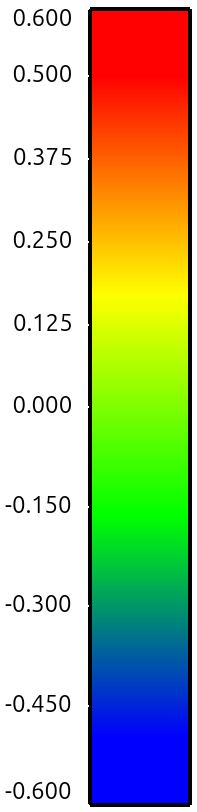
\includegraphics[width=0.98\textwidth]{img/7_versuche/cam_anzahl/scala.png}

    \end{subfigure}
    \begin{subfigure}{0.27\textwidth}
        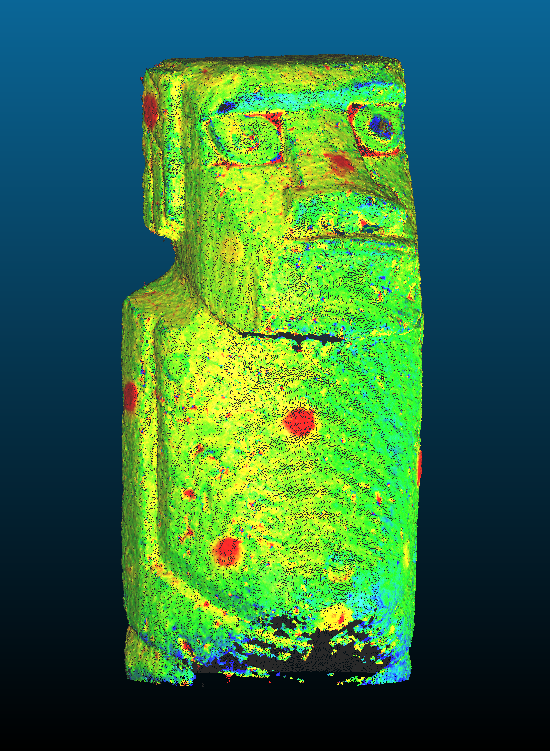
\includegraphics[width=1\textwidth]{img/7_versuche/cam_anzahl/normal.png}
        \caption{Moai}
        \label{img:differenz_moai_einzel}
    \end{subfigure}
    \begin{subfigure}{0.27\textwidth}
        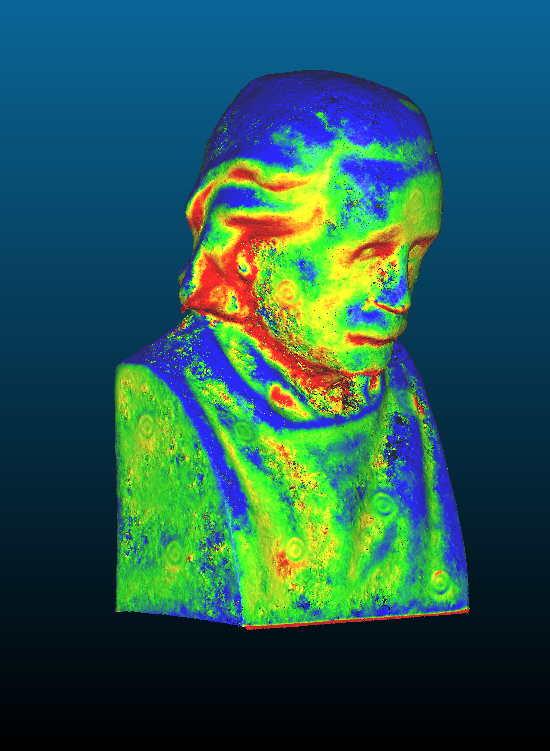
\includegraphics[width=1\textwidth]{img/7_versuche/einstein_diff.png}
        \caption{Einstein}
        \label{img:differenz_einstein}
    \end{subfigure}
    \begin{subfigure}{0.27\textwidth}
        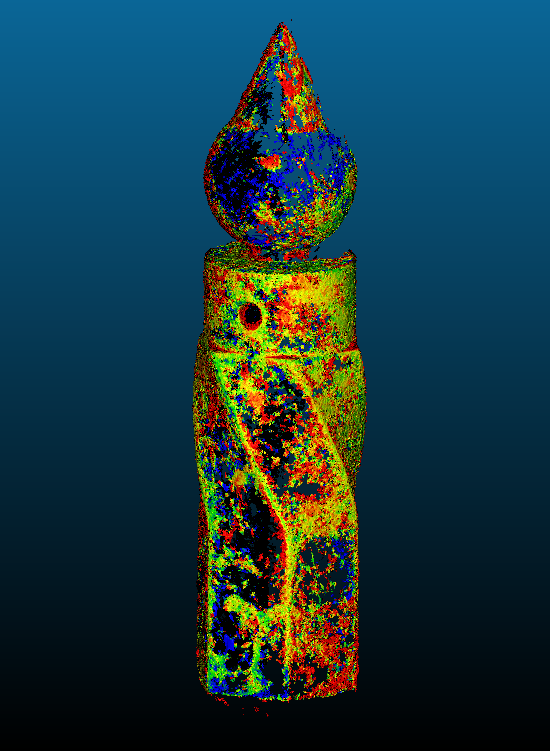
\includegraphics[width=1\textwidth]{img/7_versuche/testy_diff.png}
        \caption{Testy}
        \label{img:differenz_testy}
    \end{subfigure}
    \caption{Differenzbilder verschiedener 3D-Modelle}
    \label{img:differenz}
\end{figure}

\begin{table}
    \centering
    \caption{Ergebnisse der Genauigkeitsüberprüfung}
    \label{tab:vergleich_erg}
    \begin{tabular}{l|r|r|r}
        \toprule
                                          & Durchschnittlicher                & Mittlerer                         & Maximaler                        \\
                                          & Fehler                            & Fehler                            & Fehler                           \\
        %\midrule
        %Gesamt     & \SI{0,37}{\milli\metre}            & \SI{1,09}{\milli\metre}   & \SI{11,6}{\milli\metre}   \\  % Oberflächenmodell alt
        %gefiltert  & \SI{0,20}{\milli\metre}            & \SI{0,72}{\milli\metre}   & \SI{1,9}{\milli\metre}    \\
        \midrule
        Moai                              & \SI{-0,024}{\milli\metre}         & \SI{0,159}{\milli\metre}          & \SI{2,57}{\milli\metre}          \\  % Vertices neu
        ...ohne Bereiche der Marker       & \SI{-0,038}{\milli\metre}         & \SI{0,140}{\milli\metre}          & \SI{2,59}{\milli\metre}          \\  % Vertices neu
        \textit{...manuell mit Nikon D90} & \textit{\SI{0,255}{\milli\metre}} & \textit{\SI{0,154}{\milli\metre}} & \textit{\SI{1,33}{\milli\metre}} \\
        \midrule
        Einstein                          & \SI{0,001}{\milli\metre}          & \SI{0,356}{\milli\metre}          & \SI{-3,64}{\milli\metre}         \\
        \midrule
        Testy                             & \SI{-0,047}{\milli\metre}         & \SI{0,644}{\milli\metre}          & \SI{11,56}{\milli\metre}         \\
        \bottomrule
    \end{tabular}
\end{table}


\section{Nutzung eines Drehtellers}
\label{s:drehteller}
Statt die reelle Zahl der Kameras zu erhöhen, kann auch ein Drehteller genutzt werden, sodass jede Kamera mehr als ein Bild zur Erfassung des Objektes liefert.

\subsection{Durchführung}
Hierzu wurde ein einfacher manueller Drehteller genutzt (IKEA SNUDDA). Dieser wurde mit Passpunkten beklebt und weist ansonsten eine texturreiche Naturholzoberfläche auf (siehe \autoref{img:drehteller_moai}). Die Daten wurden in Metashape weiterverarbeitet und die einzelnen Aufnahmeschritte über die Passpunkte und die Punktwolke zusammengerechnet. Die Ergebnisse wurden mit denen des Streifenprojektionssystems und den Aufnahmen ohne Drehteller verglichen.

\begin{figure}
    \centering
    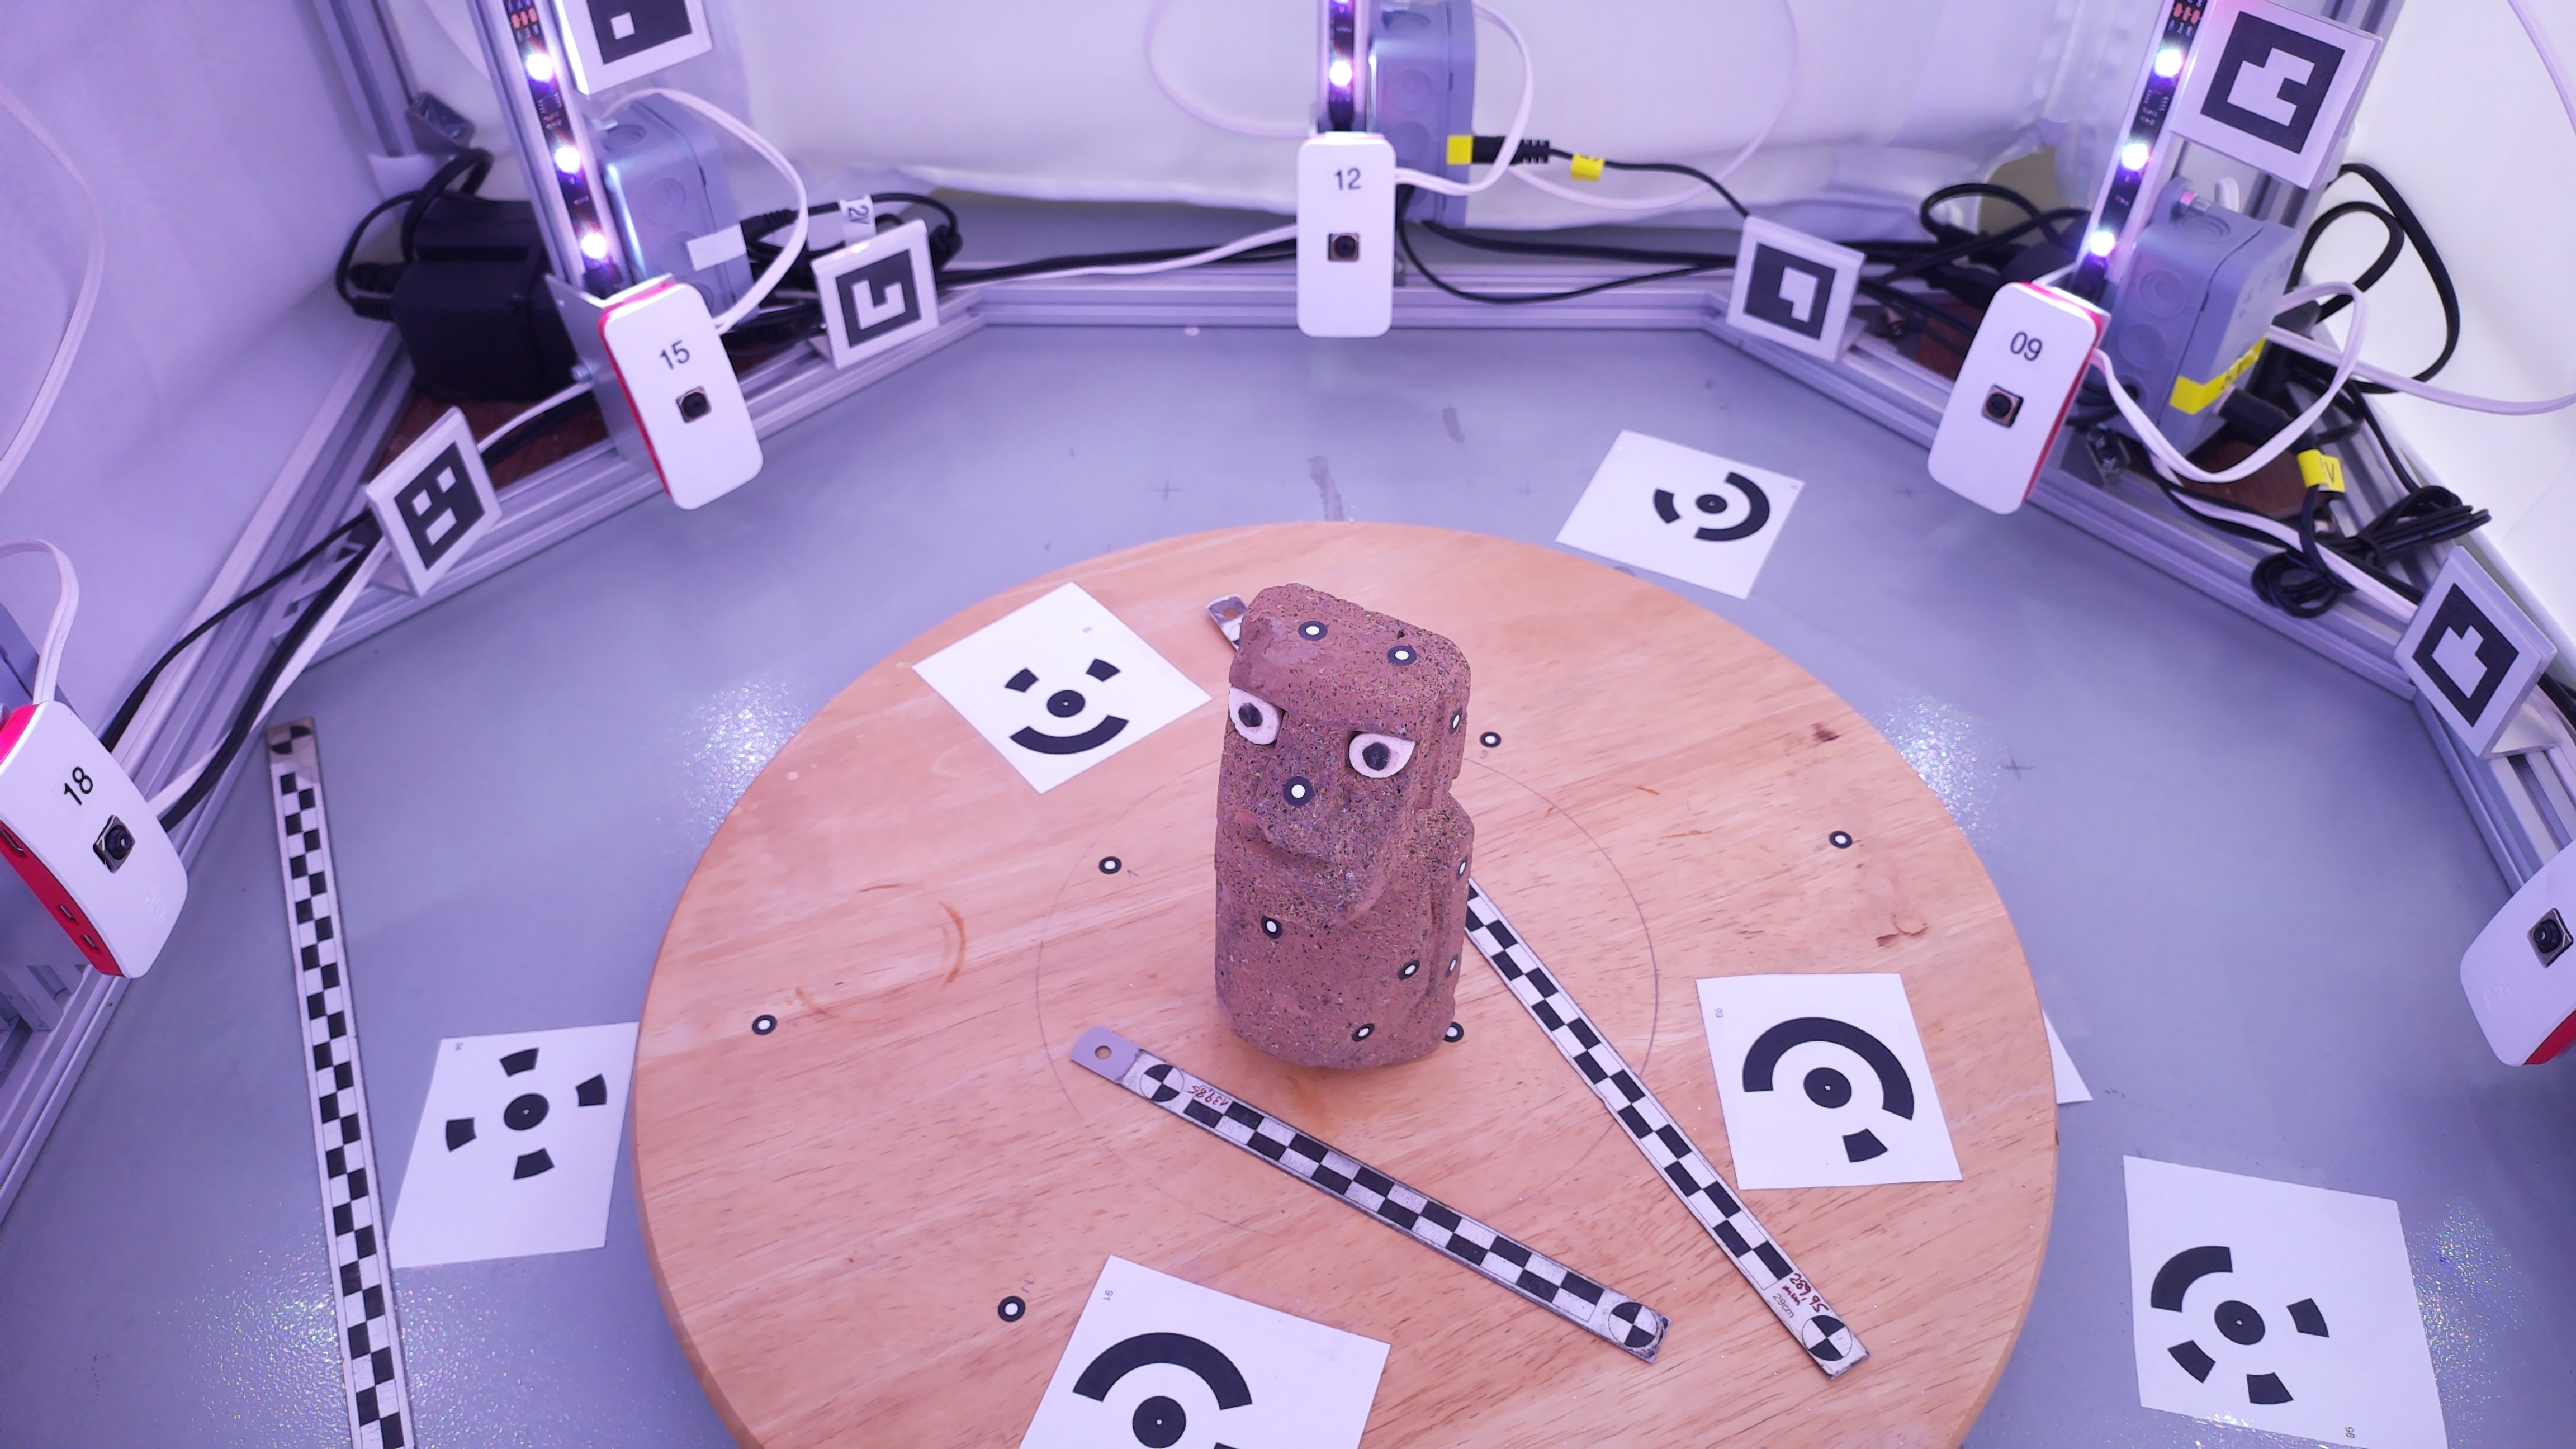
\includegraphics[width=0.8\textwidth]{img/7_versuche/drehteller_moai.jpg}
    \caption{Drehteller mit Moai-Figur im Prototypen (aufgenommen von einem der verbauten Raspberry Camera Module 3)}
    \label{img:drehteller_moai}
\end{figure}

\subsection{Ergebnisse}

In \autoref{img:differenz_moai_drehteller} ist das Differenzbild des Moai zu sehen. Es zeigt sich, dass die Genauigkeit des Modells mit Drehteller deutlich besser ist, als die des Modells ohne Drehteller (siehe \autoref{img:differenz_moai_einzel}). Auch ist die visuelle Vollständigkeit deutlich höher, die nach unten gerichteten Flächen sind auch erfasst und passen gut zu dem Modell des Streifenprojektionssystems. Die Anzahl der Punkte hat sich nicht relevant verändert -- im Vergleich zu dem vollständigen Modell der Spiegelreflexkamera zeigt sich, dass über die Punktanzahl selbst keine sinnvollen Aussagen zur Abdeckung getroffen werden können.

Der geringe durchschnittliche Fehler ist auf die automatische Anpassung des Maßstabes zurückzuführen.

Die Ergebnisse sind in \autoref{tab:vergleich_drehteller} zusammengefasst.

\begin{table}
    \centering
    \caption{Ergebnisse der unter Anpassung des Maßstabes durchgeführten Genauigkeitsüberprüfung}
    \label{tab:vergleich_drehteller}
    \begin{tabular}{l|r|r|r|r}
        \toprule
                        & Durchschnittlicher       & Mittlerer               & Maximaler              & Punktanzahl \\
                        & Fehler                   & Fehler                  & Fehler                 &             \\
        \midrule
        ohne Drehteller & \SI{-0,03}{\milli\metre} & \SI{0,22}{\milli\metre} & \SI{2,0}{\milli\metre} & 3,3 Mio.    \\
        mit Drehteller  & \SI{-0,03}{\milli\metre} & \SI{0,15}{\milli\metre} & \SI{1,6}{\milli\metre} & 3,4 Mio.    \\
        Nikon D90       & \SI{0,03}{\milli\metre}  & \SI{0,17}{\milli\metre} & \SI{1,2}{\milli\metre} & 0,05 Mio.   \\
        \bottomrule
    \end{tabular}
\end{table}

\begin{figure}
    \centering
    \begin{subfigure}{0.10\textwidth}
        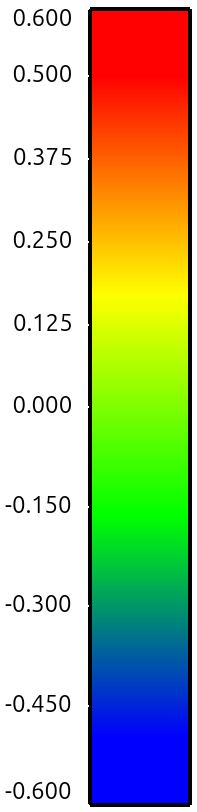
\includegraphics[width=0.98\textwidth]{img/7_versuche/cam_anzahl/scala.png}
    \end{subfigure}
    \begin{subfigure}{0.85\textwidth}
        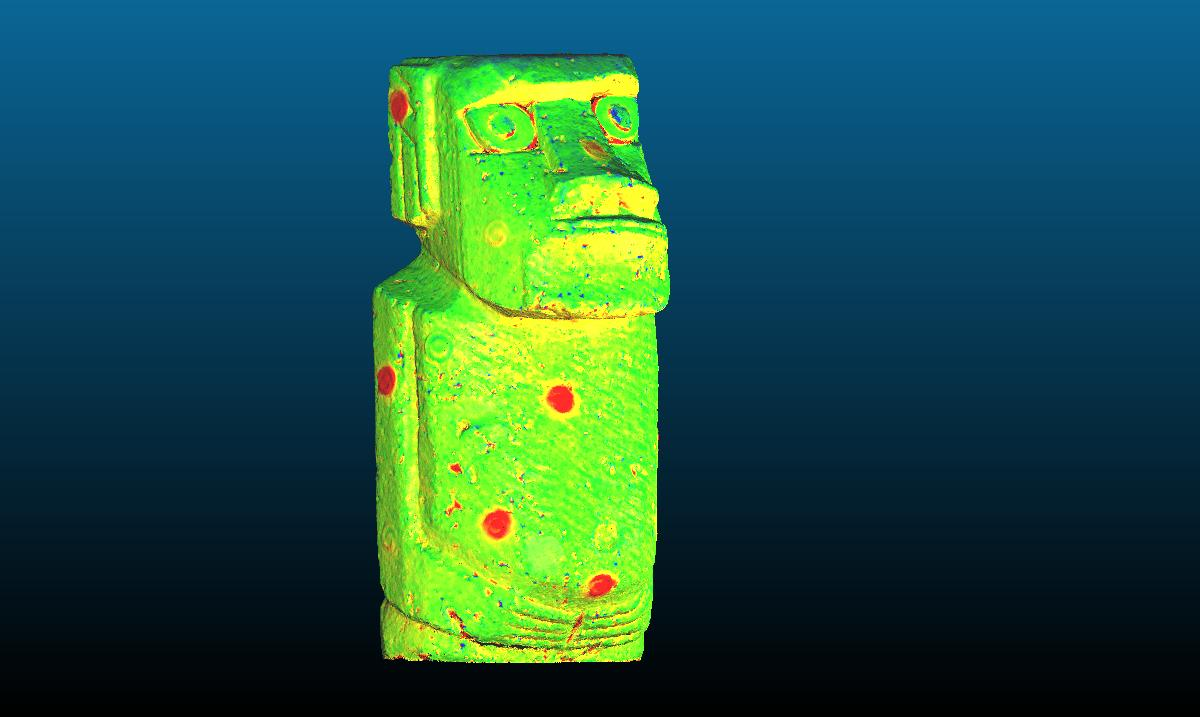
\includegraphics[width=0.98\textwidth]{img/7_versuche/moai_fehler_drehteller.jpg}
    \end{subfigure}
    \caption{Differenzbild des Moai}
    \label{img:differenz_moai_drehteller}
\end{figure}



\section{Evaluation der Kameraanzahl}
\label{s:kameraanzahl}
Die Kameras machen einen großen Teil des (Kosten-)Aufwandes zur Realisierung des Projektes aus. Es soll daher in diesem Schritt geprüft werden, ob die Anzahl der Kameras auch reduziert werden kann und die mindestens für die Testobjekte notwendige Anzahl bestimmt werden. Entsprechend \autoref{s:drehteller} wird auch der Einsatz des Drehtellers statt mehr Kameras geprüft.

\subsection{Durchführung}
Um abzuschätzen, wie viele Kameras für eine gute Genauigkeit notwendig sind, wurden verschiedene Konfigurationen getestet. Dazu wurde der Moai aus \autoref{s:genauigkeitsueberpruefung} verwendet und in Agisoft Metashape verschiedene Kameras deaktiviert und das 3D-Modell neu berechnet. Die Ergebnisse wurden wieder mit dem Streifenprojektionssystem ATOS 5 verglichen. Als weitere Parameter wurden die Abdeckung und die Richtigkeit der Punktwolke bestimmt. Die Verteilung der jeweils genutzten Kameras ist in \autoref{img:ueberblick_cam_anzahl} dargestellt. Die pink dargestellten Punkte stellen jeweils die aktiven Kameras dar.

Als Ausgleich für fehlende Kameras wurde auch nochmal der Drehteller aus der vorherigen Untersuchung verwendet und geprüft, wie viele Kameras durch den Drehteller ersetzt werden können. Die verwendeten Drehungen sind der Tabelle und den Bildern jeweils in der Form [Anzahl Aufnahmen]$\times$[Betrag der Drehung] zu entnehmen. Die Drehungen sind zusätzlich auch in \autoref{img:ueberblick_cam_anzahl} dargestellt. Jeder Strich steht für eine Aufnahme mit den aktiven Kameras. Beispielsweise zeigt die Abbildung \autoref{img:jedeZweiteKamera} zwei Striche auf dem angedeuteten Drehteller. Diese entsprechen zwei Aufnahmen mit einer Drehung zwischen den beiden Aufnahmen von $\frac{1}{8}$, also hier \ang{45}.

Zur Bestimmung des Maßstabes wurden die Daten automatisiert bestmöglich an die Referenzdaten angepasst. Die Passpunkte wurden daher hier nur als Verknüpfungspunkte genutzt und nicht zur Bestimmung des Maßstabes.


\begin{figure}
    \begin{subfigure}{0.48\textwidth}
        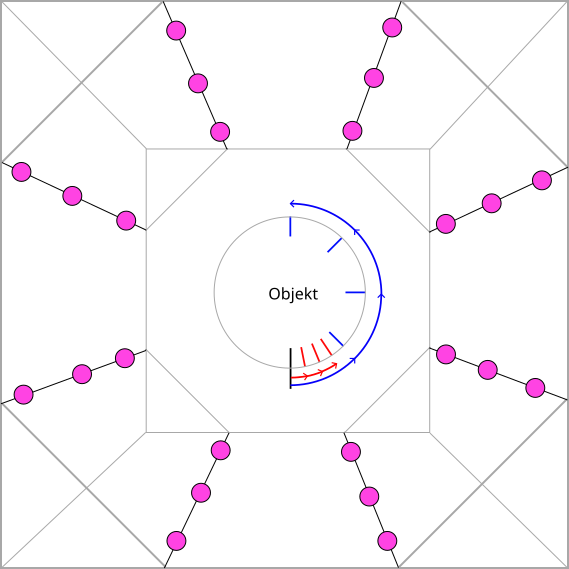
\includegraphics[width=0.95\linewidth]{img/7_versuche/kameraPosition/blick_von_oben_alle.png}
        \caption{
            24 Kameras,\\
            $4 \times \frac{1}{32}$-Drehung (rot)\\
            $5 \times \frac{1}{8}$-Drehung (blau)
        }
        \label{img:alleKameras}
    \end{subfigure}
    \begin{subfigure}{0.48\textwidth}
        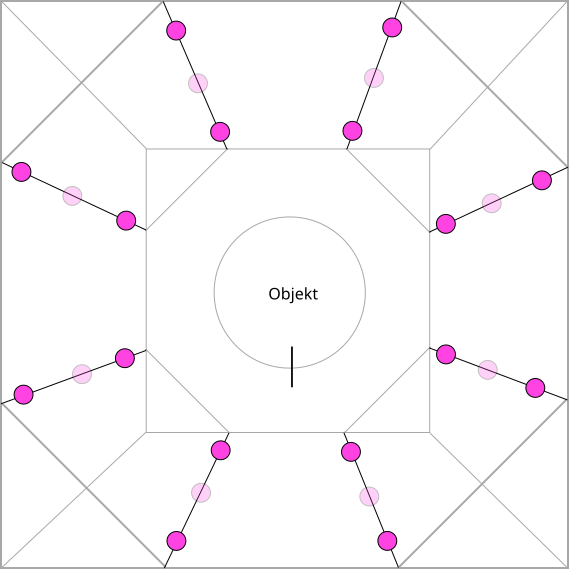
\includegraphics[width=0.95\linewidth]{img/7_versuche/kameraPosition/blick_von_oben_zweidrittel.png}
        \caption{
            16 Kameras \\
            keine Drehung \\
            ~
        }
        \label{img:2von3kameras}
    \end{subfigure}
    \par\bigskip
    \begin{subfigure}{0.48\textwidth}
        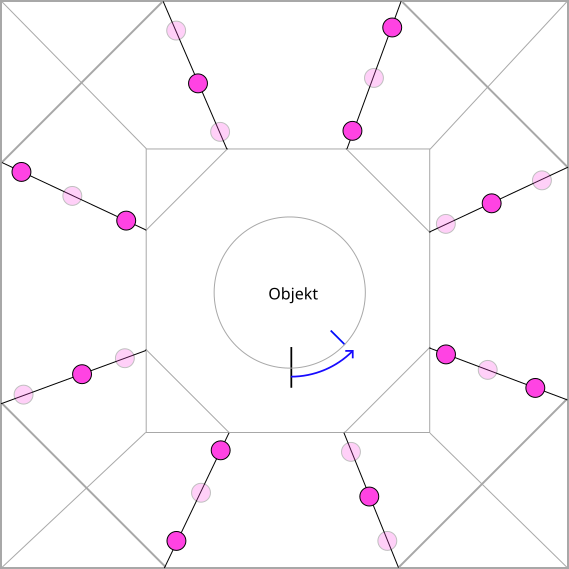
\includegraphics[width=0.95\linewidth]{img/7_versuche/kameraPosition/blick_von_oben_jedeZweite.png}
        \caption{
            12 Kameras, \\
            $2 \times \frac{1}{8}$-Drehung (blau)
        }
        \label{img:jedeZweiteKamera}
    \end{subfigure}
    \begin{subfigure}{0.48\textwidth}
        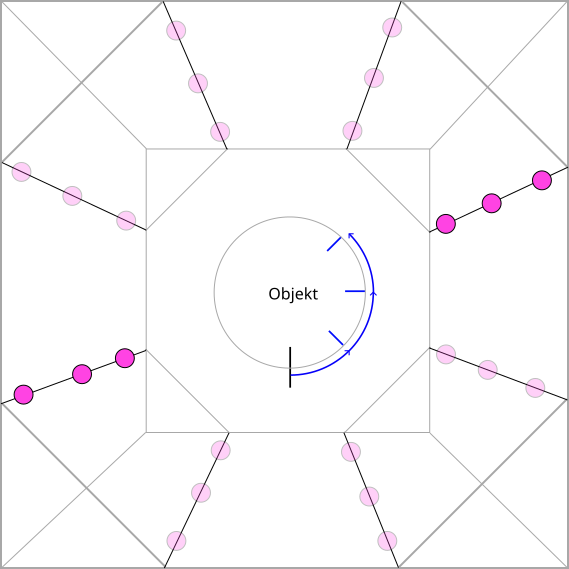
\includegraphics[width=0.95\linewidth]{img/7_versuche/kameraPosition/blick_von_oben_ebene.png}
        \caption{
            6 Kameras, \\
            $4 \times \frac{1}{8}$-Drehung (blau)
        }
        \label{img:kameras_ebene}
    \end{subfigure}
    \caption{Positionierung der Kameras und verwendete Positionen des Drehtellers, Blick von oben auf das System}
    \label{img:ueberblick_cam_position}
\end{figure}


\subsection{Ergebnisse}
Wie zu erwarten nahm die Abdeckung und die Qualität der Punktwolke ab, je weniger Kameras verwendet wurden. Bei einer Aufnahme mit allen 24 Kameras wurde die Oberfläche (ohne Boden) zu \SI{93}{\percent} abgedeckt (siehe \autoref{img:moai_normal}). Bei einer Aufnahme mit 18 Kameras (siehe \autoref{img:moai_2von3}) waren es nur noch \SI{68}{\percent} und bei 12 Kameras (siehe \autoref{img:moai_jede2K}) noch \SI{54}{\percent}.  Schon bei 18 Kameras war der Moai kaum mehr zu erkennen, bei 12 war die Erkennbarkeit nicht mehr gegeben. Die Anzahl der Kameras scheint also für dieses Objekt angebracht zu sein, sofern kein Drehteller genutzt wird.

Unter Nutzung des Drehtellers mit einer Drehung um eine Achtel-Drehung konnten sogar mit nur der Hälfte der Kameras (siehe \autoref{img:moai_jede2K_mitDrehung}) ein ähnliches bzw. sogar minimal besseres Ergebnis erzielt werden, als bei der einfachen Aufnahme mit 24 Kameras. Bei der Verwendung von nur 6 Kameras in einer Ebene, so wie es bei der Planung des Rahmens auch einmal angedacht war, brachte auch die Verwendung des Drehtellers mit 4 Positionen kein brauchbares Ergebnis im direkten Anlauf (siehe \autoref{img:moai_eineEbene}). Erst durch manuelles mehrfaches Verarbeiten der Daten und die Nutzung weiterer Passpunkte konnte die Genauigkeit und Abdeckung auf ein ähnliches Niveau wie bei 12 Kameras und zwei Aufnahmen gebracht werden (siehe \autoref{img:moai_eineEbene_mitMarkern}) - dafür aber mit einem deutlich höheren personellen und technischen Aufwand.

Im Vergleich des Parameters der Richtigkeit zeigt sich ein ähnliches Bild: Auch hier schneiden die Aufnahmen mit wenig Bildern und ohne Drehteller deutlich schlechter ab. Der Parameter zeigt, dass zwar die Punktwolken immer ähnlich viele Punkte haben, jedoch der Großteil davon außerhalb der 1-mm-Genauigkeit liegt. Die Aufnahmen mit Drehteller schneiden hier deutlich besser ab, als die ohne, erreichen aber nicht die Qualität der Aufnahmen mit 24 Kameras, vor allem nicht der Aufnahmen mit 24 Kameras und Nutzung des Drehtellers.

Die Ergebnisse sind in \autoref{tab:vergleich_anzahl_drehteller} zusammengefasst. Zum Vergleich sind auch die Ergebnisse der Nutzung des Drehtellers mit 24 Kameras aufgeführt - einmal mit feinen Drehungen von $\frac{1}{32}$ (siehe \autoref{img:moai_feinschritt}) und einmal mit groben Drehungen von $\frac{1}{8}$ (siehe \autoref{img:moai_grobschritt}). \autoref{img:ueberblick_cam_anzahl} zeigt die Abweichungen der jeweiligen Punktwolken von den Referenzdaten in grafischer Form.

\begin{table}
    \centering
    \caption{Ergebnisse mit unterschiedlicher Kameraanzahl und teilweise Nutzung eines Drehtellers}
    \label{tab:vergleich_anzahl_drehteller}
    \resizebox{\textwidth}{!}{%
        \begin{tabular}{l|l|l|l|l|l|l|l|l}
            \textbf{Art}   & \textbf{\begin{tabular}[c]{@{}l@{}}Kamera-\\ Anzahl\end{tabular}} & \textbf{Drehungen}       & \textbf{Bilder}          & \textbf{\begin{tabular}[c]{@{}l@{}}Mittlerer\\ Fehler\end{tabular}} & \textbf{\begin{tabular}[c]{@{}l@{}}Maximaler\\ Fehler\end{tabular}} & \textbf{Punktanzahl} & \textbf{Abdeckung}                         & \textbf{Richtigkeit}                       \\ \hline
            ATOS 5         & \cellcolor[HTML]{EEEEEE}                                          & \cellcolor[HTML]{EEEEEE} & \cellcolor[HTML]{EEEEEE} & \cellcolor[HTML]{EEEEEE}                                            & \cellcolor[HTML]{EEEEEE}                                            & 346830               & \SI{100,0}{\percent}                       & \SI{100,0}{\percent}                       \\ \hline
            Automatik      & 24                                                                & 1                        & 24                       & \SI{0,18}{\milli\metre}                                             & \SI{2,52}{\milli\metre}                                             & 628727               & \SI{93,1}{\percent}                        & \SI{99,9}{\percent}                        \\
            Feinschritt    & 24                                                                & 4 x $\frac{1}{32}$       & 96                       & \SI{0,14}{\milli\metre}                                             & \SI{1,42}{\milli\metre}                                             & 758364               & \SI{100,2}{\percent}                       & \SI{100,0}{\percent}                       \\
            Grobschritt    & 24                                                                & 5 x $\frac{1}{8}$        & 120                      & \SI{0,16}{\milli\metre}                                             & \cellcolor[HTML]{EEEEEE}                                            & 777533               & \SI{98,8}{\percent}                        & \SI{100,0}{\percent}                       \\ \hline
            2 von 3        & 16                                                                & 1                        & 16                       & {\color[HTML]{FF0000} \SI{1,20}{\milli\metre}}                      & {\color[HTML]{FF0000} \SI{7,74}{\milli\metre}}                      & 596979               & {\color[HTML]{FF0000} \SI{68,4}{\percent}} & {\color[HTML]{FF0000} \SI{70,4}{\percent}} \\ \hline
            jede zweite K. & 12                                                                & 1                        & 12                       & \SI{0,49}{\milli\metre}                                             & \SI{4,01}{\milli\metre}                                             & 346830               & {\color[HTML]{FF0000} \SI{54,9}{\percent}} & \SI{94,1}{\percent}                        \\
            … mit Drehung  & 12                                                                & 2 x $\frac{1}{8}$        & 24                       & \SI{0,25}{\milli\metre}                                             & \SI{1,44}{\milli\metre}                                             & 760538               & \SI{95,7}{\percent}                        & \SI{99,8}{\percent}                        \\ \hline
            eine Ebene     & 6                                                                 & 4 x $\frac{1}{8}$        & 24                       & {\color[HTML]{FF0000} \SI{1,57}{\milli\metre}}                      & \SI{1,44}{\milli\metre}                                             & 753062               & {\color[HTML]{FF0000} \SI{77,8}{\percent}} & {\color[HTML]{FF0000} \SI{68,6}{\percent}} \\
            … mit Markern  & 6                                                                 & 5 x $\frac{1}{8}$        & 30                       & \SI{0,29}{\milli\metre}                                             & \SI{2,50}{\milli\metre}                                             & 640810               & \SI{94,2}{\percent}                        & \SI{98,9}{\percent}
        \end{tabular}
    }
\end{table}

\begin{figure}
    \centering
    \begin{subfigure}{0.30\textwidth}
        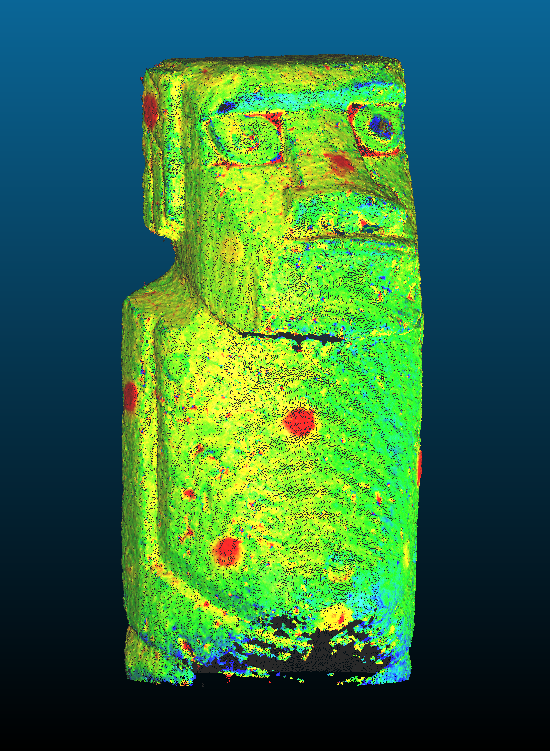
\includegraphics[width=1\linewidth]{img/7_versuche/cam_anzahl/normal.png}
        \centering
        \caption{
            24 Kameras,\\
            keine Drehung\\
            $\rightarrow 24$ Bilder
        }
        \label{img:moai_normal}
    \end{subfigure}
    \begin{subfigure}{0.30\textwidth}
        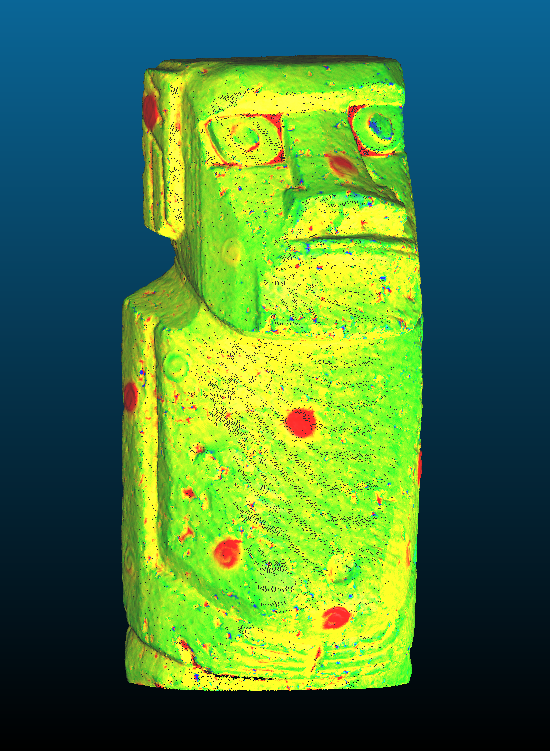
\includegraphics[width=1\linewidth]{img/7_versuche/cam_anzahl/feinschritt.png}
        \centering
        \caption{
            24 Kameras,\\
            $4 \times \frac{1}{32}$-Drehung\\
            $\rightarrow 96$ Bilder
        }
        \label{img:moai_feinschritt}
    \end{subfigure}
    \begin{subfigure}{0.30\textwidth}
        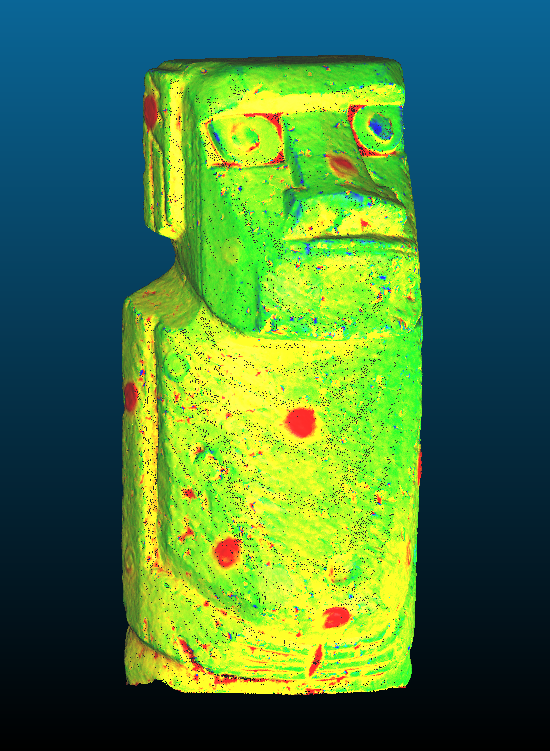
\includegraphics[width=1\linewidth]{img/7_versuche/cam_anzahl/allCamerasWithMask.png}
        \centering
        \caption{
            24 Kameras,\\
            $5 \times \frac{1}{8}$-Drehung\\
            $\rightarrow 120$ Bilder
        }
        \label{img:moai_grobschritt}
    \end{subfigure}
    \begin{subfigure}{0.30\textwidth}
        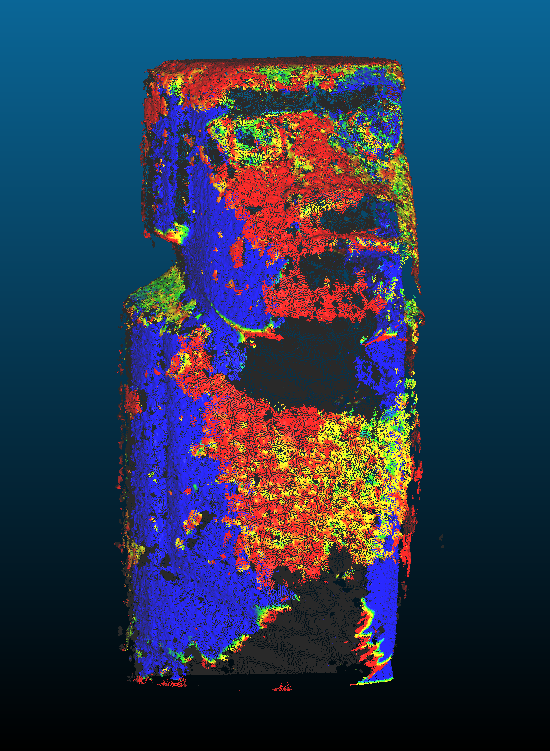
\includegraphics[width=1\linewidth]{img/7_versuche/cam_anzahl/twothirds2.png}
        \centering
        \caption{
            16 Kameras,\\
            keine Drehung\\
            $\rightarrow 16$ Bilder
        }
        \label{img:moai_2von3}
    \end{subfigure}
    \begin{subfigure}{0.30\textwidth}
        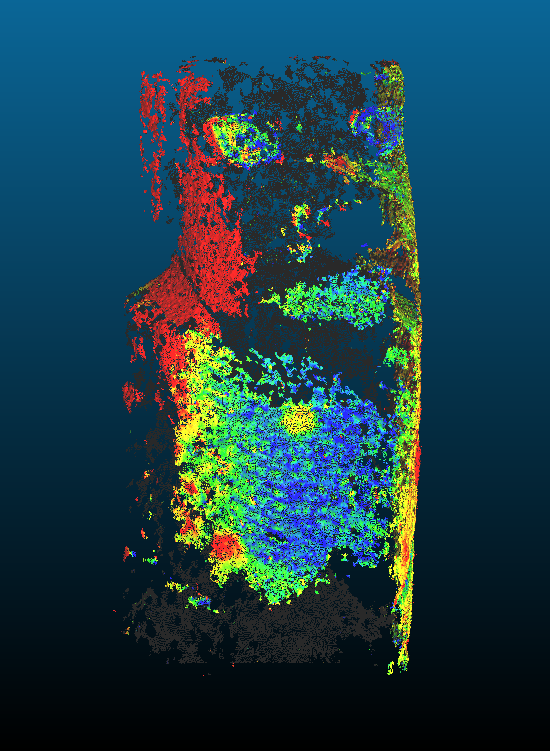
\includegraphics[width=1\linewidth]{img/7_versuche/cam_anzahl/second2.png}
        \centering
        \caption{
            12 Kameras,\\
            keine Drehung\\
            $\rightarrow 12$ Bilder
        }
        \label{img:moai_jede2K}
    \end{subfigure}
    \begin{subfigure}{0.30\textwidth}
        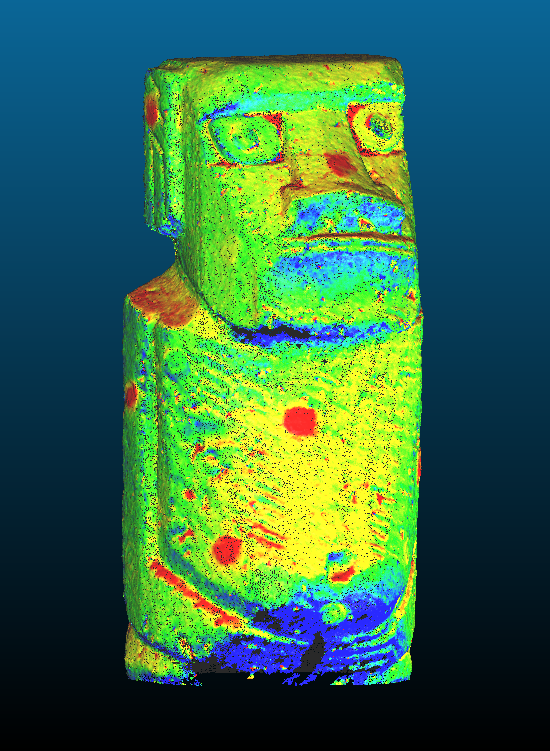
\includegraphics[width=1\linewidth]{img/7_versuche/cam_anzahl/everysecondoneturn.png}
        \centering
        \caption{
            12 Kameras,\\
            $2 \times \frac{1}{8}$-Drehung\\
            $\rightarrow 24$ Bilder
        }
        \label{img:moai_jede2K_mitDrehung}
    \end{subfigure}
    \begin{subfigure}{0.30\textwidth}
        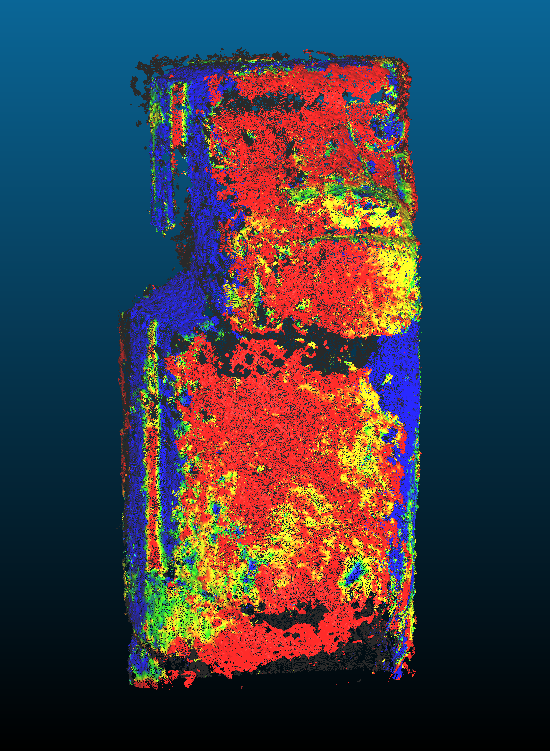
\includegraphics[width=1\linewidth]{img/7_versuche/cam_anzahl/justOneRow4Turns.png}
        \centering
        \caption{
            6 Kameras,\\
            $4 \times \frac{1}{8}$-Drehung\\
            $\rightarrow 24$ Bilder
        }
        \label{img:moai_eineEbene}
    \end{subfigure}
    \begin{subfigure}{0.30\textwidth}
        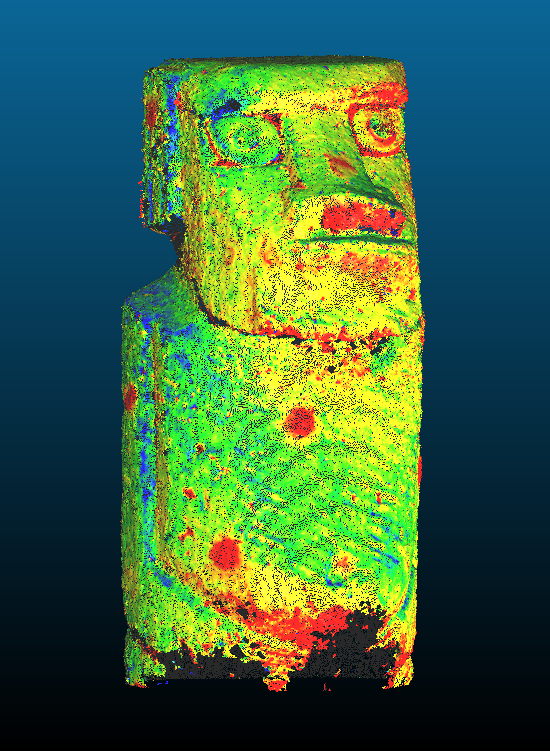
\includegraphics[width=1\linewidth]{img/7_versuche/cam_anzahl/justOneRow4TurnsRedefined.png}
        \centering
        \caption{
            6 Kameras,\\
            $4 \times \frac{1}{8}$-Drehung\\
            $\rightarrow 24$ Bilder + Marker
        }
        \label{img:moai_eineEbene_mitMarkern}
    \end{subfigure}
    \begin{subfigure}{0.30\textwidth}
        \centering
        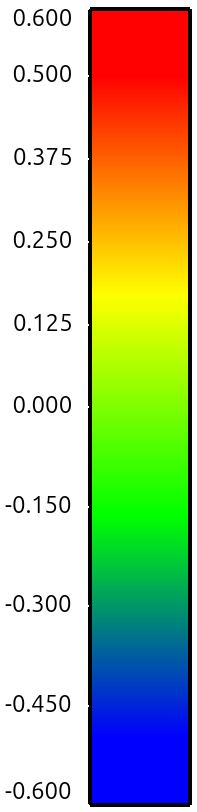
\includegraphics[width=0.33\linewidth]{img/7_versuche/cam_anzahl/scala.png}
        \caption{Skala\\~\\~}
    \end{subfigure}

    \caption{Abweichungen der jeweiligen Punktwolken von den Referenzdaten}
    \label{img:ueberblick_cam_anzahl}
\end{figure}


\section{Zusammenfassung}
Das System erreichte die vorgesehene Genauigkeit - sie lag je nach Testobjekt bei \SI{0,1}{\milli\metre} - \SI{0,5}{\milli\metre}.
Die Anzahl von 24 Kameras war für die meisten getesteten Objekte ausreichend. Experimente mit weniger Kameras führten schnell zu einer schwachen Abdeckung des Objektes und somit zu fehlenden Bereichen in der Punktwolke. Der Einsatz eines Drehtellers kann die Anzahl der notwendigen Kameras reduzieren, jedoch ist die Verarbeitung der Daten deutlich aufwändiger. Der Einsatz des Drehtellers zur weiteren Genauigkeitssteigerung ist aber durchaus sinnvoll, wenn die Anzahl der Kameras nicht erhöht werden kann oder soll.


\biblio
\end{document}